\section{Protocol cycles: when order matters}
\label{sec:ex_holonomy}

This experiment isolates P$_3$, the protocol cycle. If the effect of an interface move depends on \emph{when} it is made, then sequences of moves can reach outcomes that single moves cannot distinguish. The signature to look for is control that is equal at one step and larger over several steps.

\subsection{Setup}
We compare the reference ring world of \cref{tab:configs} with and without the protocol; the two configurations are otherwise identical. With the protocol on, LEFT and RIGHT move the agent one site at even phase and two sites at odd phase, so the effect of a move depends on the phase at which it is made. With the protocol off, every move is one site. In both regimes movement costs one unit, REPAIR is free, there is no income, the ledger holds at most two units, damage flips with probability $0.1$, and moves slip with probability $0.2$.

Safety is $r\ge1$. In both regimes the viability kernel contains all 64 states with $r\ge 1$, since the free REPAIR action leaves position and ledger unchanged. For each horizon $H=1,\dots,5$ we compute feasible empowerment to the position $y$, with all three actions as channel inputs and the initial-budget rule of \cref{sec:engine}, for the same 32 start states sampled from $\K$ (seed $0$), and report the median.

\subsection{Result: equal at one step, separated from two steps on}
\Cref{fig:protocol_horizon} shows the medians (in bits):
\begin{center}
\small
\begin{tabular}{@{}lccccc@{}}
\toprule
$H$ & 1 & 2 & 3 & 4 & 5 \\
\midrule
Protocol on  & 1.050 & 1.725 & 1.742 & 1.846 & 1.846 \\
Protocol off & 1.050 & 1.210 & 1.288 & 1.288 & 1.288 \\
\bottomrule
\end{tabular}
\end{center}
At $H=1$ the two regimes coincide. Here the reason can be checked directly: from any start state, the one-step channels of the two regimes differ only in whether the moved-to positions are one or two sites away, so they are the same channel up to a relabelling of outputs and have the same capacity. This is a property of these particular channels, not a general theorem about protocols. From $H=2$ on, the protocol regime has higher median empowerment, and the gap is largest (about $0.56$~bits) at $H=4$ and $5$. Neither curve can decrease with the horizon, because appending the free REPAIR action to every sequence leaves both the cost and the final position unchanged. Longer sequences can produce more distinguishable distributions of the final position, sometimes by reaching additional positions; the protocol curve gains more.

\begin{figure}[t]
  \centering
  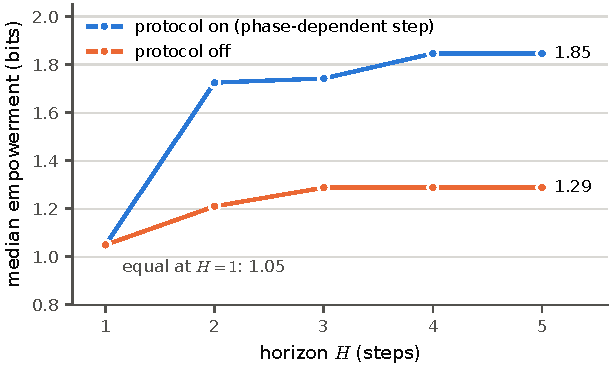
\includegraphics[width=0.72\linewidth]{figures/fig_protocol_horizon.pdf}
  \caption{Median feasible empowerment (bits) to the outside position $y$ as a function of horizon, with and without the phase-dependent step. Medians are over the same 32 start states sampled from the viability kernel. The curves coincide at $H=1$ and separate from $H=2$ on.}
  \label{fig:protocol_horizon}
\end{figure}

\subsection{A direct test of order dependence}
The medians aggregate many effects. For a sharper test we fix one start state, $s^\star=(y=0,\ u=0,\ \phi=1,\ r=2)$, and compare the two orders of the same moves, $\alpha=(\mathrm{RIGHT},\mathrm{LEFT})$ and $\beta=(\mathrm{LEFT},\mathrm{RIGHT})$. Both cost two units and are affordable from $r=2$. \Cref{tab:holonomy_witness} reports the total variation distance between the resulting distributions of $y$.

\begin{table}[t]
\centering
\small
\begin{tabular}{@{}lcc@{}}
\toprule
Damage noise & protocol on & protocol off \\
\midrule
$p_{\mathrm{flip}}=0.1$ (as in the exhibit) & 0.672 & 0.096 \\
$p_{\mathrm{flip}}=0$ (matched, noise-free damage) & 0.640 & 0.000 \\
\bottomrule
\end{tabular}

\caption{Total variation distance between the outside-position distributions produced by RIGHT-then-LEFT and LEFT-then-RIGHT from $s^\star=(y=0,u=0,\phi=1,r=2)$. Exact values: $84/125$ and $12/125$ with damage noise, $16/25$ and $0$ without it. The slip probability is $0.2$ in all four cases.}
\label{tab:holonomy_witness}
\end{table}

With the damage noise of the main experiment, order matters in both regimes ($0.672$ with the protocol, $0.096$ without). The second effect has nothing to do with the protocol: if damage occurs between the two moves, it reverses the direction of the second move, and the resulting displacement depends on which move came first. When damage noise is set to zero and everything else is kept, the protocol-free regime becomes exactly order-independent (distance $0$), while the protocol regime keeps a large order effect ($0.64$). This matched, noise-free pair isolates the protocol as the source of order dependence; the noisy pair shows that order effects in the full system also have other sources.

\subsection{Interpretation}
In \SBT\ terms, the protocol cycle is neither memory (P$_5$) nor budget (P$_6$): it concerns the order in which interface moves compose. In this substrate it leaves one-step control unchanged and enlarges multi-step control, without changing the viability kernel or the packaging lens. The agent's interface becomes more expressive over longer horizons; it can cause more distinguishable outcomes with the same moves and the same budget.
